\documentclass[border=1pt]{standalone}
\usepackage{tikz}
\usepackage{luatexja}

\begin{document}
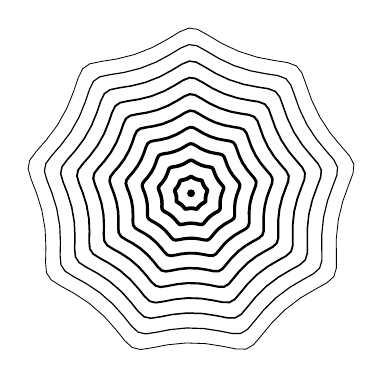
\begin{tikzpicture}
    \foreach \r in {0.2, 0.4, ..., 2.0} {
        % 外側に行くほど線の太さを変え、少しずつ揺らす
        \pgfmathsetmacro{\jitter}{0.05 * \r}
        \draw[black, line width={1.5pt - 0.6pt*\r}] 
            plot[domain=0:360, samples=72] 
            ({\r*cos(\x) + \jitter*sin(8*\x)}, {\r*sin(\x) + \jitter*cos(8*\x)});
    }
    \fill[black] (0,0) circle (0.05);
\end{tikzpicture}
\end{document}
